% Chapter Template
\chapter{Conclusiones} % Main chapter title
\label{Capitulo5} % Change X to a consecutive number; for referencing this chapter elsewhere, use \ref{ChapterX}
\lhead{\emph{Conclusiones}}

%----------------------------------------------------------------------------------------
%	SECTION 1
%----------------------------------------------------------------------------------------
Dentro de la descripción de la Hipotesis se menciona como objetivo lograr una mejora posterior al aplicar el procedimiento CTIS mediante filtrados diversos que puedieran eliminar ruido de las imágenes hiperespectrales resultantes. 

Mediante la utilización Mosaico Bayer y método de Malvar (vea \ref{capMalvar}) previo a la generación de imágenes de cubo hiperespectral, se pudo permitir que el resultado tuviera una mejora significante.
Después de obtener dicho resultado se aplica el método CTIS para obtener las imágenes y a estas imágenes se le aplica el desenfoque (vea capítulo \ref{CapBlur}) y la nitidez (véa \ref{capSharpender}) como último paso en el proceso.

Posterior a ello se aplicaron las series de Daubichies (vea la sección \ref{rDau}) que fueron descartados ya que no se presento algúna mejora notable al ser aplicado dejando el desenfoque y la nitidez como pasos definitivos.

La forma en que se comprobo la mejora fue visual, ya que por ser se tenían imagenes sin ruido con las cuales validar. Esto debido a que se trabajó directamente con imagenes abstraidas de la camara \ref{} con estructura CTIS.

Gracias a la aportación dada el presente proyecto se podrá dar una mejora con la cual será posible obtener un acercamiento a un producto con mayor madurez capaz de dar como resultado imagenes con mayor calidad(conservando detalles y eliminando ruido).


\begin{figure}[h]
\begin{center}$
\begin{array}{lll}
\subfloat[Original]{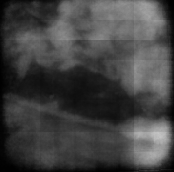
\includegraphics[scale=1.5]{./images/RESULTS/compare870/original.png}}&
\subfloat[MSB]{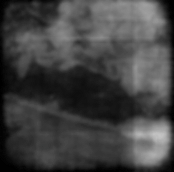
\includegraphics[scale=1.125]{./images/RESULTS/compare870/MSB.png}}
\end{array}$
\end{center}

\caption{Proceso para MSBD en extracción 870-845.}
\label{pics:process}
\end{figure}